% =====================================================================
% Section 7: Results and Discussion
% Requires in the preamble: \usepackage{booktabs, graphicx}
% Figures: figures/fig_walk_forward.pdf, figures/fig_delay.pdf
% All numbers come from results/*.csv in the project repository.
% =====================================================================

\section{Results and Discussion}
\label{sec:results}

\subsection{Evaluation Protocol}
\label{sec:protocol}

All results in this section use one shared pipeline and one backtest, so that the
models are directly comparable. Three properties of the protocol matter for reading
the numbers.

\begin{enumerate}
  \item \textbf{Three-way chronological split with purging.} The 1,030,551 aligned
  snapshots are split 70/15/15 into training (04-07 11:34 to 04-15 20:00 UTC), validation
  (to 04-17 14:57) and test (to 04-19 09:54). A row is used as a target only if its whole
  label window $[t, t+h]$ lies inside its own split. Early stopping uses the
  \emph{validation} loss.
  \item \textbf{Trading rules are chosen on validation only.} Every tunable trading
  parameter (the confidence threshold $\theta$ and the hysteresis enter/exit levels) is
  selected by validation Sharpe and then applied once to the test split. An earlier draft
  of this project selected $\theta$ on the test split; those numbers are not reported
  here.
  \item \textbf{Fee-aware, non-overlapping backtest.} A position $q_t\in\{-1,0,+1\}$ (full
  capital, no leverage) is held for exactly $h$ seconds and earns the mid-price return
  $r_{t,h}$. Steps do not overlap. The net step return is
  $q_t r_{t,h} - c\,|q_t - q_{t-1}|$ with $c = 1.5$\,bp, so a reversal pays twice, and
  wealth compounds multiplicatively. Execution is at the mid-price of the same snapshot
  the features come from. Section~\ref{sec:delay} relaxes this assumption.
\end{enumerate}

Three trading rules map the predicted class probabilities $(p_\downarrow, p_0, p_\uparrow)$
to positions: \emph{argmax} trades every prediction; \emph{threshold} goes long if
$p_\uparrow > \theta$, short if $p_\downarrow > \theta$, and is otherwise flat;
\emph{hysteresis} opens a position when its class probability exceeds an \emph{enter}
level, keeps it while that probability stays above a lower \emph{exit} level, and reverses
directly on a strong opposite signal. A LightGBM classifier on the current second's
features only serves as a non-deep baseline.

% ---------------------------------------------------------------------
\subsection{Classification Performance}
\label{sec:classification}

Table~\ref{tab:classification} reports test classification metrics at the 10-second
horizon. All four models reach 41--44\% accuracy, which is \emph{no better than always
predicting Flat} (43.1\% of test labels). Accuracy is therefore not informative here.
Directional F1, the macro F1 over the Down and Up classes, does show a weak but
consistent directional signal of 0.44--0.47. The Transformer has the highest directional
F1 (0.466), but the gap to the other models is small: LightGBM, which sees only the
current second, reaches 0.465. The sequence architectures add little classification
skill beyond the hand-crafted features.

\begin{table}[htbp]
\centering
\caption{Test classification metrics, 10-second horizon, main split
(154,544 test targets). DirF1 = macro F1 over Down and Up. Always predicting Flat
gives an accuracy of 0.431.}
\label{tab:classification}
\begin{tabular}{lcccccc}
\toprule
 & \multicolumn{2}{c}{Full (38F)} & \multicolumn{2}{c}{No PCA (88F)} & \multicolumn{2}{c}{No Market (23F)} \\
\cmidrule(lr){2-3}\cmidrule(lr){4-5}\cmidrule(lr){6-7}
Model & Acc & DirF1 & Acc & DirF1 & Acc & DirF1 \\
\midrule
Residual CNN      & 0.445 & 0.454 & 0.444 & 0.448 & 0.443 & 0.437 \\
BiLSTM            & 0.434 & 0.447 & 0.434 & 0.449 & 0.436 & 0.445 \\
Transformer       & 0.437 & \textbf{0.466} & 0.434 & 0.464 & 0.436 & 0.456 \\
LightGBM baseline & 0.409 & 0.465 & 0.408 & 0.461 & 0.413 & 0.444 \\
\bottomrule
\end{tabular}
\end{table}

Across feature sets, removing the market-state block (No Market) lowers directional F1
for every model (by 0.002--0.020), while replacing PCA factors with the raw 60 LOB
columns (No PCA) changes it by less than 0.007. Cross-asset features help slightly; PCA
compression neither helps nor hurts.

% ---------------------------------------------------------------------
\subsection{Trading Performance on the Main Split}
\label{sec:trading}

Table~\ref{tab:trading} reports the test backtest at the 10-second horizon. Buy-and-hold
loses 6.5\% over the test window, which contains the 18 April sell-off (maximum drawdown
$-14.8\%$).

\begin{table}[htbp]
\centering
\caption{Test returns at the 10-second horizon (15,457 non-overlapping steps, 1.5\,bp
fee). $\theta$ and the hysteresis levels are chosen on validation. Turnover = total
$\sum_t|q_t-q_{t-1}|$. Buy-and-hold: $-6.52\%$.}
\label{tab:trading}
\begin{tabular}{llrrrrr}
\toprule
 & & Argmax & \multicolumn{2}{c}{Threshold} & \multicolumn{2}{c}{Hysteresis} \\
\cmidrule(lr){4-5}\cmidrule(lr){6-7}
Model & Features & Return & Return & Turnover & Return & Turnover \\
\midrule
Residual CNN & Full      & $-40.1\%$ & $+0.72\%$ & 28  & $\mathbf{+26.8\%}$ & 2,249 \\
Residual CNN & No PCA    & $-40.3\%$ & $-0.35\%$ & 42  & -- & -- \\
Residual CNN & No Market & $-42.2\%$ & $-0.71\%$ & 62  & -- & -- \\
BiLSTM       & Full      & $-48.6\%$ & $-0.16\%$ & 96  & $+4.5\%$ & 428 \\
BiLSTM       & No PCA    & $-46.9\%$ & $+0.27\%$ & 22  & -- & -- \\
BiLSTM       & No Market & $-46.5\%$ & $-0.12\%$ & 54  & -- & -- \\
Transformer  & Full      & $-42.8\%$ & $+0.32\%$ & 152 & $+3.5\%$ & 284 \\
Transformer  & No PCA    & $-39.7\%$ & $-0.06\%$ & 24  & -- & -- \\
Transformer  & No Market & $-42.5\%$ & $+0.05\%$ & 30  & -- & -- \\
LightGBM     & Full      & $-39.3\%$ & $+0.08\%$ & 20  & $+6.3\%$ & 974 \\
LightGBM     & No PCA    & $-42.6\%$ & $-0.21\%$ & 280 & $+17.1\%$ & 1,922 \\
LightGBM     & No Market & $-42.5\%$ & $-0.34\%$ & 114 & $-0.9\%$ & 1,039 \\
\bottomrule
\end{tabular}
\end{table}

\paragraph{Argmax.} Trading every prediction loses 39--49\% for every model and feature
set. Even with a non-trivial directional F1, the expected move per 10-second step is far
smaller than the 1.5\,bp paid on each position change.

\paragraph{Threshold.} A confidence threshold chosen on validation ($\theta = 0.55$--$0.85$)
almost stops the models from trading: 20--280 position changes over 1.8 days, with test
returns between $-0.7\%$ and $+0.7\%$. With so few trades these results are not
distinguishable from zero. In particular, the earlier draft's CNN result of $+2.7\%$
(Sharpe 31) does not survive once $\theta$ is selected out of sample.

\paragraph{Hysteresis.} Separating the entry and exit levels changes the picture. The
model now stays in a position through small dips in confidence instead of paying to close
and reopen it. Five of the six hysteresis runs turn positive. The CNN earns $+26.8\%$
(Sharpe 62, maximum drawdown $-6.4\%$). On this split, the result is not a single lucky
configuration. Both long positions ($+15.1\%$) and short positions ($+22.9\%$) contribute,
before $-14.1\%$ of fees. Each of the three test days is positive ($+3.6\%$, $+16.9\%$,
$+3.5\%$). Every neighbouring (enter, exit) pair within $\pm 0.05$ also stays positive
($+14.1\%$ to $+49.0\%$). The LSTM ($+3.0\%$ to $+14.7\%$ over the same neighbourhood)
and the Transformer ($+0.0\%$ to $+11.9\%$) are positive on every test day as well, with
far less trading.

% ---------------------------------------------------------------------
\subsection{Effect of the Prediction Horizon}
\label{sec:horizon}

A natural way to beat the fee is to predict further ahead, since price moves grow with
the horizon while the fee does not. We rebuilt the labels for $h \in \{30, 60, 300\}$
seconds, with the Up/Down threshold raised to the round-trip cost of 3\,bp, and retrained
every model on the Full feature set (Table~\ref{tab:horizon}).

\begin{table}[htbp]
\centering
\caption{Directional F1 and hysteresis test return by prediction horizon (Full feature
set, main split). ``Flat'' = share of Flat labels in the test set, which equals the
accuracy of always predicting Flat. Buy-and-hold $\approx -6.6\%$ at every horizon.}
\label{tab:horizon}
\begin{tabular}{rc cc cc cc cc}
\toprule
 & & \multicolumn{2}{c}{CNN} & \multicolumn{2}{c}{BiLSTM} & \multicolumn{2}{c}{Transformer} & \multicolumn{2}{c}{LightGBM} \\
\cmidrule(lr){3-4}\cmidrule(lr){5-6}\cmidrule(lr){7-8}\cmidrule(lr){9-10}
$h$ & Flat & DirF1 & Hyst. & DirF1 & Hyst. & DirF1 & Hyst. & DirF1 & Hyst. \\
\midrule
10\,s  & 0.431 & 0.454 & $+26.8\%$ & 0.447 & $+4.5\%$ & 0.466 & $+3.5\%$  & 0.465 & $+6.3\%$ \\
30\,s  & 0.359 & 0.413 & $+0.1\%$  & 0.426 & $+0.7\%$ & 0.437 & $+1.0\%$  & 0.446 & $+13.3\%$ \\
60\,s  & 0.244 & 0.436 & $+8.3\%$  & 0.445 & $+4.0\%$ & 0.416 & $-0.3\%$  & 0.466 & $+8.6\%$ \\
300\,s & 0.107 & 0.420 & $-4.4\%$  & 0.447 & $-3.9\%$ & 0.372 & $-12.3\%$ & 0.476 & $-2.4\%$ \\
\bottomrule
\end{tabular}
\end{table}

Longer horizons do not help. Accuracy rises above the Flat baseline only because Flat
labels become rare, and directional F1 stays at 0.37--0.48 at every horizon. The
apparent gains at 30 and 60 seconds come mostly from short positions during the 18 April
sell-off, and they are fragile. For LightGBM at 30 seconds, for example, the test return
over the neighbouring (enter, exit) pairs ranges from $-12.1\%$ to $+14.9\%$. At 300
seconds every hysteresis run loses money. LightGBM matches or exceeds the deep models'
directional F1 at every horizon.

% ---------------------------------------------------------------------
\subsection{Walk-Forward Evaluation}
\label{sec:walkforward}

The main split has a single 1.8-day test window. Many configurations were compared on
it, so its best result is optimistically selected. To test whether the 10-second
hysteresis result generalises, we re-ran the CNN and LightGBM on rolling folds. Each fold
trains on 5 days, validates on the next day and tests on the day after, and the window
then moves forward one day, giving six disjoint test days from 13 to 18 April. Within
each fold, the PCA basis is refitted on that fold's training days, the hysteresis levels
are chosen on its validation day, and the CNN is trained with three seeds plus a
seed-averaged ensemble. The first four test days were not used to choose this
configuration, so they are genuinely out of sample.

\begin{table}[htbp]
\centering
\caption{Walk-forward test-day returns (10-second horizon, hysteresis, 1.5\,bp fee). Each
column is one fold; a ``day'' starts at 11:34 UTC. CNN single seeds: mean of the three
seeds on each day (individual runs range from $+1.0\%$ to $+35.3\%$).}
\label{tab:walkforward}
\begin{tabular}{lrrrrrr|r}
\toprule
Test day & 04-13 & 04-14 & 04-15 & 04-16 & 04-17 & 04-18 & Mean \\
\midrule
CNN, 3-seed ensemble    & $+4.2\%$ & $+3.1\%$ & $+9.8\%$ & $+9.0\%$ & $+6.2\%$ & $+10.0\%$ & $+7.0\%$ \\
CNN, single-seed mean   & $+2.9\%$ & $+2.7\%$ & $+3.6\%$ & $+6.7\%$ & $+20.6\%$ & $+9.8\%$ & $+7.7\%$ \\
LightGBM, No PCA        & $+3.2\%$ & $+8.9\%$ & $+7.9\%$ & $+5.9\%$ & $-0.8\%$ & $+11.3\%$ & $+6.1\%$ \\
LightGBM, Full          & $-2.2\%$ & $+1.0\%$ & $+12.4\%$ & $+9.3\%$ & $-2.7\%$ & $+10.8\%$ & $+4.8\%$ \\
Buy-and-hold            & $+2.3\%$ & $-3.0\%$ & $-3.0\%$ & $+0.7\%$ & $-10.9\%$ & $+4.5\%$ & $-1.6\%$ \\
\bottomrule
\end{tabular}
\end{table}

\begin{figure}[htbp]
\centering
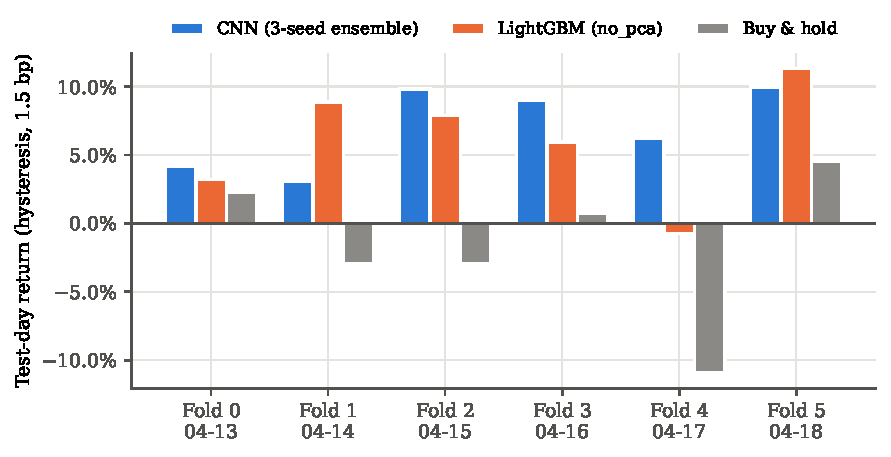
\includegraphics[width=0.85\linewidth]{figures/fig_walk_forward.pdf}
\caption{Walk-forward test-day returns of the hysteresis strategy against buy-and-hold.}
\label{fig:walkforward}
\end{figure}

Table~\ref{tab:walkforward} and Figure~\ref{fig:walkforward} show that the result is
remarkably stable \emph{under the backtest's assumptions}. All 18 single-seed CNN runs and
all six ensemble days are positive, including the four test days before the sell-off,
which were not used to choose the configuration. Compounded over the six days, the CNN
ensemble returns $+50.1\%$ against $-9.7\%$ for buy-and-hold. Seed averaging lowers the
variance: single seeds range from $+1.0\%$ to $+35.3\%$, the ensemble from $+3.1\%$ to
$+10.0\%$. LightGBM is profitable on 5 of 6 days with No PCA features and on 4 of 6 with
Full features. Directional F1 stays at 0.41--0.47 in every fold, the same level as on the
main split.

% ---------------------------------------------------------------------
\subsection{Reality Checks: Execution Delay and Data Alignment}
\label{sec:delay}

\paragraph{Execution delay.} The backtest assumes we trade at the mid-price of the very
snapshot from which the features were computed. To test this, we keep every trained model
and every validation-chosen threshold fixed and decide the position for the step starting
at second $t$ from the prediction made at second $t-d$. This uses only the saved
predictions, so no retraining is involved. Figure~\ref{fig:delay} and
Table~\ref{tab:delay} show the result.

\begin{figure}[htbp]
\centering
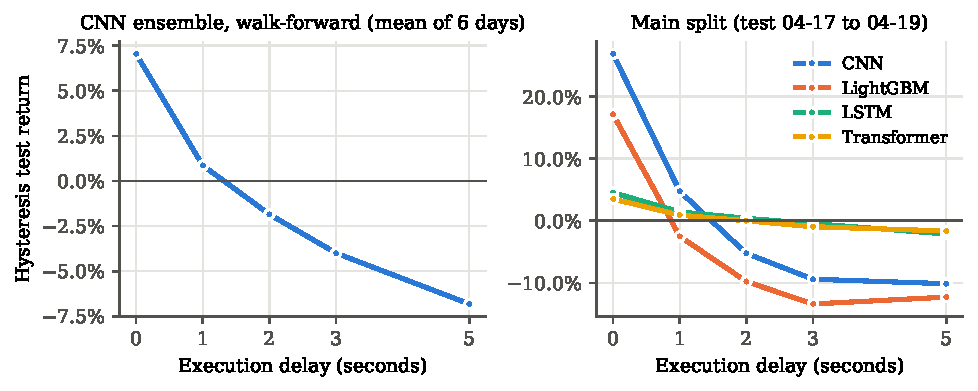
\includegraphics[width=\linewidth]{figures/fig_delay.pdf}
\caption{Hysteresis test return as a function of execution delay. Left: CNN ensemble,
mean over the six walk-forward test days. Right: all models on the main split.}
\label{fig:delay}
\end{figure}

\begin{table}[htbp]
\centering
\caption{Hysteresis test return with execution delayed by $d$ seconds (10-second horizon,
same models and thresholds). Walk-forward rows: mean over six test days (share of
positive days in brackets).}
\label{tab:delay}
\small
\begin{tabular}{lrrrrr}
\toprule
 & $d=0$ & $d=1$\,s & $d=2$\,s & $d=3$\,s & $d=5$\,s \\
\midrule
\multicolumn{6}{l}{\emph{Walk-forward (mean per test day)}} \\
CNN ensemble  & $+7.0\%$ (6/6) & $+0.9\%$ (4/6) & $-1.9\%$ (3/6) & $-4.0\%$ (2/6) & $-6.8\%$ (0/6) \\
CNN single seeds & $+7.7\%$ & $+2.3\%$ & $-1.0\%$ & $-2.9\%$ & $-4.9\%$ \\
LightGBM (Full + No PCA) & $+4.9\%$ & $-3.6\%$ & $-4.2\%$ & $-6.3\%$ & $-9.0\%$ \\
\midrule
\multicolumn{6}{l}{\emph{Main split (test 04-17 to 04-19)}} \\
CNN               & $+26.8\%$ & $+4.7\%$ & $-5.2\%$ & $-9.4\%$ & $-10.1\%$ \\
BiLSTM            & $+4.5\%$  & $+1.4\%$ & $+0.4\%$ & $-0.5\%$ & $-2.1\%$ \\
Transformer       & $+3.5\%$  & $+0.9\%$ & $+0.0\%$ & $-1.0\%$ & $-1.6\%$ \\
LightGBM, No PCA  & $+17.1\%$ & $-2.5\%$ & $-9.8\%$ & $-13.4\%$ & $-12.3\%$ \\
\bottomrule
\end{tabular}
\end{table}

For every model, most of the profit disappears with a one-second delay, and it turns
negative at two to three seconds. The models do anticipate the next move of the
mid-price, but that move happens within roughly one second of the snapshot. The LSTM and
Transformer lose less when delayed only because their validation-chosen entry levels are
higher, so they trade less. Their profit decays in the same way.

\paragraph{BTC--ETH timestamp alignment.} BTC and ETH snapshots are joined on the
floored second. Within a matched second (first 300,000 snapshots), the ETH snapshot is
recorded \emph{later} than the BTC snapshot 24.5\% of the time, by up to 0.74\,s (19.7\% of
seconds are more than 0.1\,s later). In those seconds, the ETH-based market features
contain information from slightly after the BTC mid-price they are compared with, which
is a small look-ahead in every feature set that includes market features. A delay of one
second or more removes this leak as well, which is a further reason to treat the delayed
numbers as the realistic ones.

% ---------------------------------------------------------------------
\subsection{Discussion}
\label{sec:discussion}

The results support three conclusions.

\begin{enumerate}
  \item \textbf{The models learn genuine but very short-lived order-book information.}
  Directional F1 of 0.41--0.47 is stable across architectures, feature sets, seeds and six
  walk-forward folds. Under instantaneous execution, a hysteresis rule turns this signal into
  profits that are consistent across days and robust to the choice of thresholds.
  \item \textbf{The signal is not tradable at 1-second resolution after a 1.5\,bp fee.} Its
  value is concentrated in the first second after each snapshot. With any realistic
  latency, no model, feature set, horizon or trading rule in this study has a positive
  expected return. Capturing it would require sub-second execution at the mid-price, with no
  queueing or adverse selection, which this data cannot evaluate.
  \item \textbf{Architecture matters less than evaluation design.} The three deep models
  and a LightGBM baseline that sees only the current second reach similar directional F1. The
  choices with the largest effect on reported returns are methodological: selecting
  thresholds out of sample (which removes the earlier $+2.7\%$ CNN result), separating entry
  from exit, and modelling execution delay (which removes all remaining profit).
\end{enumerate}

\paragraph{Limitations.} The data covers only 12 days in April 2021, and all test days fall in
one week that contains a single large sell-off. The backtest fills at the mid-price with a
flat fee, ignores market impact and borrowing costs for short positions, and uses
full-capital positions. The 1.5\,bp fee is lower than retail taker fees at the time. Only
the CNN and LightGBM were evaluated walk-forward; the LSTM and Transformer were checked for
execution delay on the main split only.
